%%% ----------------------------------------------------------------------
%%%%%%%%%%%%%%%%%%%%%%%%%%%%%%%%%%%%%%%%%%%%%%%%%%%%%%%%%%%%%%%%%%%%%%%%%%
\chapter[DMAT]{The Distributed Matrix Data Structure}
\label{chap:dmat}


\inspire%
{If I were again beginning my studies, I would follow the advice of Plato and start with 
mathematics.}%
{Galileo Galilei}
\vspace{0.5cm}


Before continuing, we must spend some time describing a new distributed data 
structure.  In reality, this data structure is the merging of two different 
kinds of distributed data structures, namely \emph{block distributions} and 
\emph{cyclic distributions}.  Eventually we will get to \emph{block cyclic 
distributions}, but this structure is complicated enough that it is wise to 
examine each component separately first.

\begin{figure}[ht]
        \centering
        \begin{subfigure}[b]{0.3\textwidth}
                \centering
                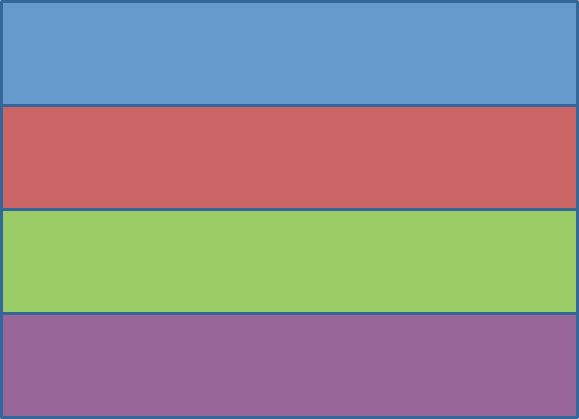
\includegraphics[height=5cm,width=\textwidth]{pbdDEMO-include/pics/dmat_block}
                \caption{Block}
        \end{subfigure}
        \hspace{.1cm}
        \begin{subfigure}[b]{0.3\textwidth}
                \centering
                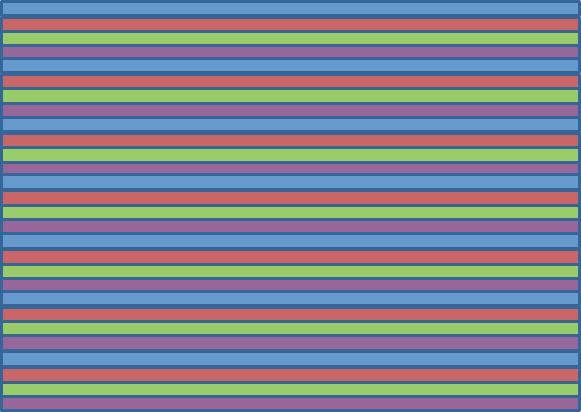
\includegraphics[height=5cm,width=\textwidth]{pbdDEMO-include/pics/dmat_cyclic}
                \caption{Cyclic}
        \end{subfigure}
        \hspace{.01cm}
        \begin{subfigure}[b]{0.3\textwidth}
                \centering
                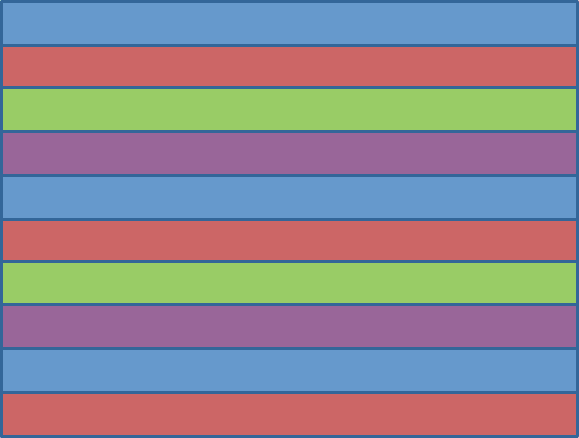
\includegraphics[height=5cm,width=\textwidth]{pbdDEMO-include/pics/dmat_blockcyclic}
                \caption{Block-Cyclic}
        \end{subfigure}
        \caption{Matrix Distribution Schemes}\label{fig:dmat1d}
\end{figure}


Figure~\ref{fig:dmat1d} shows examples of the three different distribution schemes for 4 processors.  The block scheme is simple enough; imagine chopping the matrix into nearly equal blocks and distributing those blocks to different processors.  This can be viewed as a special case of the \code{GBD} data structure of Section~\ref{sec:gbdstruct}.  

For the cyclic distribution scheme, one can imagine taking each row (or column) of a matrix and sending the first to one processor, the second to the next, and so on until all processors are exhausted; if the data is not exhausted, then one merely cycles back through the processors, continuing in this fashion until all of the matrix has been distributed.

Finally, the block-cyclic decomposition is the obvious blending of these two schemes, so that each of the former becomes a special case of this new type.  Here, we can imagine chopping the matrix up into blocks, but the blocks are not (necessarily) so large that they use up the entire matrix.  Once we use up all of the blocks, we use the cyclic data distribution scheme to cycle back through our processors, only using (potentially) blocks of more than one row at a time.  From this light, a block-cyclic distribution where the block size is large enough to get all of the data in one cycle is also a block distribution, and a block-cyclic distribution where the blocks are taking just one row at a time is also a cyclic distribution.

The obvious analogue to Figure~\ref{fig:dmat1d} for distributing by column is also possible, but there is a much more important --- and complicated --- generalization of this scheme.  Above, we were thinking of the aggregate of processors as essentially being in a vector, or lying on a one-dimensional line.  However, we can extend this to two-dimensional grids of processors as well.  
\begin{figure}[ht]
        \centering
        \begin{subfigure}[b]{0.3\textwidth}
                \centering
                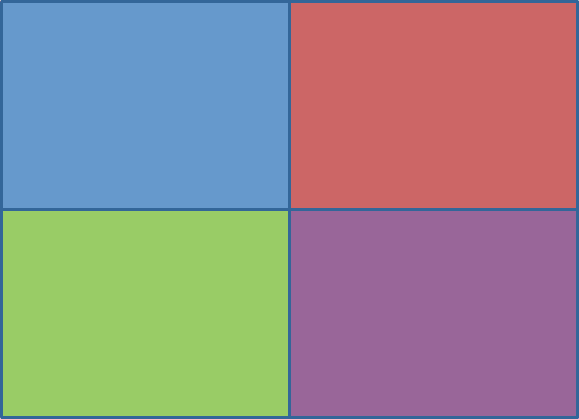
\includegraphics[height=5cm,width=\textwidth]{pbdDEMO-include/pics/dmat_block2d}
                \caption{2d Block}
        \end{subfigure}%
        \hspace{.1cm}
        \begin{subfigure}[b]{0.3\textwidth}
                \centering
                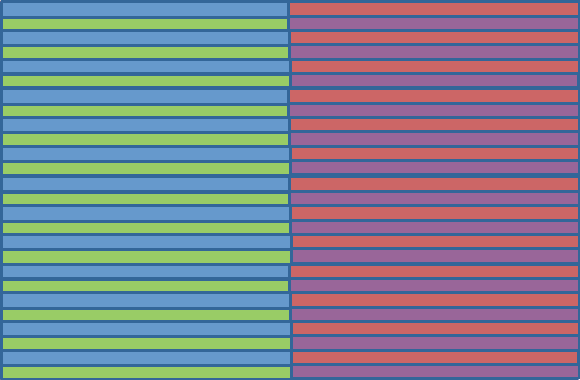
\includegraphics[height=5cm,width=\textwidth]{pbdDEMO-include/pics/dmat_cyclic2d}
                \caption{2d Cyclic}
        \end{subfigure}
        \hspace{.01cm}
        \begin{subfigure}[b]{0.3\textwidth}
                \centering
                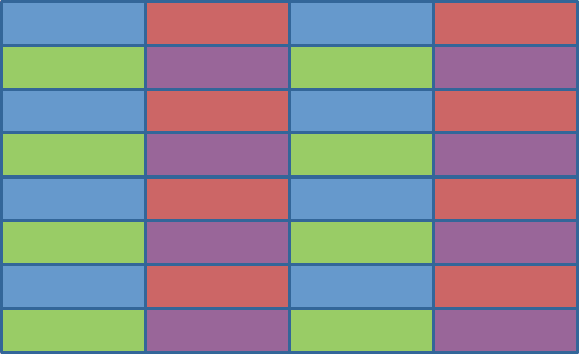
\includegraphics[height=5cm,width=\textwidth]{pbdDEMO-include/pics/dmat_blockcyclic2d}
                \caption{2d Block-Cyclic}
        \end{subfigure}
        \caption{Matrix Distribution Schemes Onto a 2-Dimensional Grid}\label{fig:dmat2d}
\end{figure}
Figure~\ref{fig:dmat2d} shows how the extension to a 2-dimensional grid of processors, still with just 4 processors, only here, we are assuming that they form a $2\times 2$ grid.  This data structure is a generalization of the 1-dimensional block-cyclic distribution, and so it is a generalization of 1-dimensional block and 1-dimensional cyclic distributions as well.

The data structure can get quite complicated, especially when there are many processors involved.
\begin{table}[ht]
        \centering
        \begin{subfigure}[b]{0.23\textwidth}
                \centering
              $\left[\begin{tabular}{llllll}
                  0 & 1 & 2 & 3 & 4 & 5
                \end{tabular}\right]$
                \caption{$1\times 6$}
        \end{subfigure}
        \begin{subfigure}[b]{0.23\textwidth}
                \centering
                $\left[\begin{tabular}{lll}
                  0 & 1 & 2\\
                  3 & 4 & 5
                \end{tabular}\right]$
                \caption{$2\times 3$}
        \end{subfigure}%
        \begin{subfigure}[b]{0.23\textwidth}
                \centering
              $\left[\begin{tabular}{ll}
                  0 & 1 \\
                  2 & 3\\
                  4 & 5
                \end{tabular}\right]$
                \caption{$3\times 2$}
        \end{subfigure}
        \begin{subfigure}[b]{0.23\textwidth}
                \centering
              $\left[\begin{tabular}{l}
                  0 \\ 1 \\ 2 \\ 3 \\ 4 \\ 5
                \end{tabular}\right]$
                \caption{$6\times 1$}
        \end{subfigure}
        \caption{Processor Grid Shapes with 6 Processors}\label{fig:gridshapes}
\end{table}
Table~\ref{fig:gridshapes} shows the different possible grid shapes for six processors.  In general, if we have $n$ processors, then there are $\sigma_0(n)$ total possible grid shapes, where
\begin{align*}
\sigma_m(n) &= \sum_{d\ |\ n} d^m
\end{align*}
and $d\in\mathbb{N}$ (a positive integer).  Thus the grid shapes are given by:
\begin{align*}
\left( d, \frac{n}{d} \right)
\end{align*}
for each $d\ |\ n$ with $d\in\mathbb{N}$.
  
This added complication is not for pure masochism; it has some real advantages.  
For one, this 2-dimensional block-cyclic (henceforth simply referred to as 
``block-cyclic'') decomposition is the data structure employed by the state of 
the art dense linear algebra library ScaLAPACK\index{Library!ScaLAPACK}, and if 
one wishes to use this library, then the use must occur on its terms.  However, 
there are some real performance benefits to this data structure.  For many 
linear algebra operations (which includes many statistical operations, in whole 
or in part), this data structure offers an interesting balance between 
communication cost and parallelism.  For very large problems, many are surprised 
to find that communication between processors will often dwarf the computation 
overhead.  This will generally become apparent at the 10,000+ processor count 
except for the most embarrassingly parallel problems, and the cost of 
communication gets \emph{much} worse the more cores are added after that.  The 
rate at which 
this scales badly will depend a great deal on the hardware, but there is no 
machine in existence at the time of writing for which the above vague warning 
will not hold true.

Returning to the data structure, notice that since we have control over the 
processor grid shape and the blocking factor (or blocking dimension --- the 
number of rows/columns in the blocks for the block-decomposition), we can very 
directly tune the amount of parallelism, and therefore the amount of 
communication.  Make the blocks too small (say $1\times 1$, or single element 
blocks) and there will be a great deal of parallelism, in the sense that most 
processors will stay busy most of the time; but the processors will have to talk 
to each other to get \emph{anything} done.  This makes the communication cost 
skyrocket.  On the other hand, we could make the blocking factor so large in 
each dimension that it encompasses the entire matrix.  That is, the matrix would 
be stored in its entirety on a single processor.  In doing so, we entirely 
eliminate the communication, but we also elimination the parallelism.

The fact of the matter is, hard problems require data movement and 
communication.  We should strive to minimize these burdens, but not so 
myopically that we throw out the parallelism as well.  Balancing these 
parameters then becomes important, and a not entirely trivial optimization 
problem.  The \pkg{pbdDMAT} package includes defaults for each that should be 
``ok'' if you have no intuition whatsoever.  However, these defaults may not be 
well-suited to a specific problem, and knowing ahead of time how best to 
distribute the data is often more art than science.

For the remainder of this chapter, we will be examining these shapes in more depth to get a better feel for the data structure.  To do so, let us return to our old friend from Section~\ref{sec:gbdstruct}:\\
\begin{align*}
x &= \left[
      \begin{array}{lllllllll}
      x_{11} & x_{12} & x_{13} & x_{14} & x_{15} & x_{16} & x_{17} & x	_{18} & x_{19}\\
      x_{21} & x_{22} & x_{23} & x_{24} & x_{25} & x_{26} & x_{27} & x	_{28} & x_{29}\\
      x_{31} & x_{32} & x_{33} & x_{34} & x_{35} & x_{36} & x_{37} & x	_{38} & x_{39}\\
      x_{41} & x_{42} & x_{43} & x_{44} & x_{45} & x_{46} & x_{47} & x	_{48} & x_{49}\\
      x_{51} & x_{52} & x_{53} & x_{54} & x_{55} & x_{56} & x_{57} & x	_{58} & x_{59}\\
      x_{61} & x_{62} & x_{63} & x_{64} & x_{65} & x_{66} & x_{67} & x	_{68} & x_{69}\\
      x_{71} & x_{72} & x_{73} & x_{74} & x_{75} & x_{76} & x_{77} & x	_{78} & x_{79}\\
      x_{81} & x_{82} & x_{83} & x_{84} & x_{85} & x_{86} & x_{87} & x	_{88} & x_{89}\\
      x_{91} & x_{92} & x_{93} & x_{94} & x_{95} & x_{96} & x_{97} & x	_{98} & x_{99}
      \end{array}
\right]_{9\times 9}
\end{align*}
However, we note that the \pkg{pbdDMAT} package offers numerous high-level tools for managing these structures, so that the management of distributed details can be as implicit or explicit as the user desires.

\section{Block Data Distributions}

Let us start with the 1-dimensional block data distribution.  So here, we will assume that our processor grid looks like:
\begin{align*}
\text{Processors = }
\left[
      \begin{array}{llll}
      \color{g11}0 & \color{g12}1 & \color{g13}2 & \color{g21}3
      \end{array}
\right]
\end{align*}
To block-distribute our matrix onto this 1-dimensional grid by rows, then we would have no option but to do the following:
\begin{align*}
x &= \left[
      \begin{array}{lllllllll}
      \color{g11}x_{11} & \color{g11}x_{12} & \color{g11}x_{13} & \color{g11}x_{14} & \color{g11}x_{15} & \color{g11}x_{16} & \color{g11}x_{17} & \color{g11}x_{18} & \color{g11}x_{19}\\
      \color{g11}x_{21} & \color{g11}x_{22} & \color{g11}x_{23} & \color{g11}x_{24} & \color{g11}x_{25} & \color{g11}x_{26} & \color{g11}x_{27} & \color{g11}x_{28} & \color{g11}x_{29}\\
      \color{g11}x_{31} & \color{g11}x_{32} & \color{g11}x_{33} & \color{g11}x_{34} & \color{g11}x_{35} & \color{g11}x_{36} & \color{g11}x_{37} & \color{g11}x_{38} & \color{g11}x_{39}\\\hline
      \color{g12}x_{41} & \color{g12}x_{42} & \color{g12}x_{43} & \color{g12}x_{44} & \color{g12}x_{45} & \color{g12}x_{46} & \color{g12}x_{47} & \color{g12}x_{48} & \color{g12}x_{49}\\
      \color{g12}x_{51} & \color{g12}x_{52} & \color{g12}x_{53} & \color{g12}x_{54} & \color{g12}x_{55} & \color{g12}x_{56} & \color{g12}x_{57} & \color{g12}x_{58} & \color{g12}x_{59}\\
      \color{g12}x_{61} & \color{g12}x_{62} & \color{g12}x_{63} & \color{g12}x_{64} & \color{g12}x_{65} & \color{g12}x_{66} & \color{g12}x_{67} & \color{g12}x_{68} & \color{g12}x_{69}\\\hline
      \color{g13}x_{71} & \color{g13}x_{72} & \color{g13}x_{73} & \color{g13}x_{74} & \color{g13}x_{75} & \color{g13}x_{76} & \color{g13}x_{77} & \color{g13}x_{78} & \color{g13}x_{79}\\
      \color{g13}x_{81} & \color{g13}x_{82} & \color{g13}x_{83} & \color{g13}x_{84} & \color{g13}x_{85} & \color{g13}x_{86} & \color{g13}x_{87} & \color{g13}x_{88} & \color{g13}x_{89}\\
      \color{g13}x_{91} & \color{g13}x_{92} & \color{g13}x_{93} & \color{g13}x_{94} & \color{g13}x_{95} & \color{g13}x_{96} & \color{g13}x_{97} & \color{g13}x_{98} & \color{g13}x_{99}\\
      \end{array}
\right]_{9\times 9}
\end{align*}
Notice that here, processor {\color{g21}3} receives none of the matrix.  This is so because if the block size (here, $3\times 9$) were any smaller, then we would not be able to distribute all of the data without cycling.  Similarly, if we were to distribute by column then we would have:
\begin{align*}
x &= \left[
      \begin{array}{lll|lll|lll}
      \color{g11}x_{11} & \color{g11}x_{12} & \color{g11}x_{13} & \color{g12}x_{14} & \color{g12}x_{15} & \color{g12}x_{16} & \color{g13}x_{17} & \color{g13}x_{18} & \color{g13}x_{19}\\
      \color{g11}x_{21} & \color{g11}x_{22} & \color{g11}x_{23} & \color{g12}x_{24} & \color{g12}x_{25} & \color{g12}x_{26} & \color{g13}x_{27} & \color{g13}x_{28} & \color{g13}x_{29}\\
      \color{g11}x_{31} & \color{g11}x_{32} & \color{g11}x_{33} & \color{g12}x_{34} & \color{g12}x_{35} & \color{g12}x_{36} & \color{g13}x_{37} & \color{g13}x_{38} & \color{g13}x_{39}\\
      \color{g11}x_{41} & \color{g11}x_{42} & \color{g11}x_{43} & \color{g12}x_{44} & \color{g12}x_{45} & \color{g12}x_{46} & \color{g13}x_{47} & \color{g13}x_{48} & \color{g13}x_{49}\\
      \color{g11}x_{51} & \color{g11}x_{52} & \color{g11}x_{53} & \color{g12}x_{54} & \color{g12}x_{55} & \color{g12}x_{56} & \color{g13}x_{57} & \color{g13}x_{58} & \color{g13}x_{59}\\
      \color{g11}x_{61} & \color{g11}x_{62} & \color{g11}x_{63} & \color{g12}x_{64} & \color{g12}x_{65} & \color{g12}x_{66} & \color{g13}x_{67} & \color{g13}x_{68} & \color{g13}x_{69}\\
      \color{g11}x_{71} & \color{g11}x_{72} & \color{g11}x_{73} & \color{g12}x_{74} & \color{g12}x_{75} & \color{g12}x_{76} & \color{g13}x_{77} & \color{g13}x_{78} & \color{g13}x_{79}\\
      \color{g11}x_{81} & \color{g11}x_{82} & \color{g11}x_{83} & \color{g12}x_{84} & \color{g12}x_{85} & \color{g12}x_{86} & \color{g13}x_{87} & \color{g13}x_{88} & \color{g13}x_{89}\\
      \color{g11}x_{91} & \color{g11}x_{92} & \color{g11}x_{93} & \color{g12}x_{94} & \color{g12}x_{95} & \color{g12}x_{96} & \color{g13}x_{97} & \color{g13}x_{98} & \color{g13}x_{99}\\
      \end{array}
\right]_{9\times 9}
\end{align*}
for exactly the same reason.  

If we used a 2-dimensional grid of processors, say a $2\times 2$ grid:
\begin{align*}
\text{Processors = }
\left[
      \begin{array}{ll}
      \color{g11}0 & \color{g12}1 \\ \color{g13}2 & \color{g21}3
      \end{array}
\right]
\end{align*}
then our data would be distributed as
\begin{align*}
x &= \left[
      \begin{array}{lllll|llll}
      \color{g11}x_{11} & \color{g11}x_{12} & \color{g11}x_{13} & \color{g11}x_{14} & \color{g11}x_{15} & \color{g12}x_{16} & \color{g12}x_{17} & \color{g12}x_{18} & \color{g12}x_{19}\\
      \color{g11}x_{21} & \color{g11}x_{22} & \color{g11}x_{23} & \color{g11}x_{24} & \color{g11}x_{25} & \color{g12}x_{26} & \color{g12}x_{27} & \color{g12}x_{28} & \color{g12}x_{29}\\
      \color{g11}x_{31} & \color{g11}x_{32} & \color{g11}x_{33} & \color{g11}x_{34} & \color{g11}x_{35} & \color{g12}x_{36} & \color{g12}x_{37} & \color{g12}x_{38} & \color{g12}x_{39}\\
      \color{g11}x_{41} & \color{g11}x_{42} & \color{g11}x_{43} & \color{g11}x_{44} & \color{g11}x_{45} & \color{g12}x_{46} & \color{g12}x_{47} & \color{g12}x_{48} & \color{g12}x_{49}\\
      \color{g11}x_{51} & \color{g11}x_{52} & \color{g11}x_{53} & \color{g11}x_{54} & \color{g11}x_{55} & \color{g12}x_{56} & \color{g12}x_{57} & \color{g12}x_{58} & \color{g12}x_{59}\\\hline
      \color{g13}x_{61} & \color{g13}x_{62} & \color{g13}x_{63} & \color{g13}x_{64} & \color{g13}x_{65} & \color{g21}x_{66} & \color{g21}x_{67} & \color{g21}x_{68} & \color{g21}x_{69}\\
      \color{g13}x_{71} & \color{g13}x_{72} & \color{g13}x_{73} & \color{g13}x_{74} & \color{g13}x_{75} & \color{g21}x_{76} & \color{g21}x_{77} & \color{g21}x_{78} & \color{g21}x_{79}\\
      \color{g13}x_{81} & \color{g13}x_{82} & \color{g13}x_{83} & \color{g13}x_{84} & \color{g13}x_{85} & \color{g21}x_{86} & \color{g21}x_{87} & \color{g21}x_{88} & \color{g21}x_{89}\\
      \color{g13}x_{91} & \color{g13}x_{92} & \color{g13}x_{93} & \color{g13}x_{94} & \color{g13}x_{95} & \color{g21}x_{96} & \color{g21}x_{97} & \color{g21}x_{98} & \color{g21}x_{99}\\
      \end{array}
\right]_{9\times 9}
\end{align*}




\section{Cyclic Data Distributions}

Proceeding as in the previous section, we would cyclically distribute this matrix by row onto the 1-dimensional processor grid as:
\begin{align*}
x &= \left[
      \begin{array}{lllllllll}
      \color{g11}x_{11} & \color{g11}x_{12} & \color{g11}x_{13} & \color{g11}x_{14} & \color{g11}x_{15} & \color{g11}x_{16} & \color{g11}x_{17} & \color{g11}x_{18} & \color{g11}x_{19}\\\hline
      \color{g12}x_{21} & \color{g12}x_{22} & \color{g12}x_{23} & \color{g12}x_{24} & \color{g12}x_{25} & \color{g12}x_{26} & \color{g12}x_{27} & \color{g12}x_{28} & \color{g12}x_{29}\\\hline
      \color{g13}x_{31} & \color{g13}x_{32} & \color{g13}x_{33} & \color{g13}x_{34} & \color{g13}x_{35} & \color{g13}x_{36} & \color{g13}x_{37} & \color{g13}x_{38} & \color{g13}x_{39}\\\hline
      \color{g21}x_{41} & \color{g21}x_{42} & \color{g21}x_{43} & \color{g21}x_{44} & \color{g21}x_{45} & \color{g21}x_{46} & \color{g21}x_{47} & \color{g21}x_{48} & \color{g21}x_{49}\\\hline
      \color{g11}x_{51} & \color{g11}x_{52} & \color{g11}x_{53} & \color{g11}x_{54} & \color{g11}x_{55} & \color{g11}x_{56} & \color{g11}x_{57} & \color{g11}x_{58} & \color{g11}x_{59}\\\hline
      \color{g12}x_{61} & \color{g12}x_{62} & \color{g12}x_{63} & \color{g12}x_{64} & \color{g12}x_{65} & \color{g12}x_{66} & \color{g12}x_{67} & \color{g12}x_{68} & \color{g12}x_{69}\\\hline
      \color{g13}x_{71} & \color{g13}x_{72} & \color{g13}x_{73} & \color{g13}x_{74} & \color{g13}x_{75} & \color{g13}x_{76} & \color{g13}x_{77} & \color{g13}x_{78} & \color{g13}x_{79}\\\hline
      \color{g21}x_{81} & \color{g21}x_{82} & \color{g21}x_{83} & \color{g21}x_{84} & \color{g21}x_{85} & \color{g21}x_{86} & \color{g21}x_{87} & \color{g21}x_{88} & \color{g21}x_{89}\\\hline
      \color{g11}x_{91} & \color{g11}x_{92} & \color{g11}x_{93} & \color{g11}x_{94} & \color{g11}x_{95} & \color{g11}x_{96} & \color{g11}x_{97} & \color{g11}x_{98} & \color{g11}x_{99}\\
      \end{array}
\right]_{9\times 9}
\end{align*}
and by column:
\begin{align*}
x &= \left[
      \begin{array}{l|l|l|l|l|l|l|l|l}
      \color{g11}x_{11} & \color{g12}x_{12} & \color{g13}x_{13} & \color{g21}x_{14} & \color{g11}x_{15} & \color{g12}x_{16} & \color{g13}x_{17} & \color{g21}x_{18} & \color{g11}x_{19}\\
      \color{g11}x_{21} & \color{g12}x_{22} & \color{g13}x_{23} & \color{g21}x_{24} & \color{g11}x_{25} & \color{g12}x_{26} & \color{g13}x_{27} & \color{g21}x_{28} & \color{g11}x_{29}\\
      \color{g11}x_{31} & \color{g12}x_{32} & \color{g13}x_{33} & \color{g21}x_{34} & \color{g11}x_{35} & \color{g12}x_{36} & \color{g13}x_{37} & \color{g21}x_{38} & \color{g11}x_{39}\\
      \color{g11}x_{41} & \color{g12}x_{42} & \color{g13}x_{43} & \color{g21}x_{44} & \color{g11}x_{45} & \color{g12}x_{46} & \color{g13}x_{47} & \color{g21}x_{48} & \color{g11}x_{49}\\
      \color{g11}x_{51} & \color{g12}x_{52} & \color{g13}x_{53} & \color{g21}x_{54} & \color{g11}x_{55} & \color{g12}x_{56} & \color{g13}x_{57} & \color{g21}x_{58} & \color{g11}x_{59}\\
      \color{g11}x_{61} & \color{g12}x_{62} & \color{g13}x_{63} & \color{g21}x_{64} & \color{g11}x_{65} & \color{g12}x_{66} & \color{g13}x_{67} & \color{g21}x_{68} & \color{g11}x_{69}\\
      \color{g11}x_{71} & \color{g12}x_{72} & \color{g13}x_{73} & \color{g21}x_{74} & \color{g11}x_{75} & \color{g12}x_{76} & \color{g13}x_{77} & \color{g21}x_{78} & \color{g11}x_{79}\\
      \color{g11}x_{81} & \color{g12}x_{82} & \color{g13}x_{83} & \color{g21}x_{84} & \color{g11}x_{85} & \color{g12}x_{86} & \color{g13}x_{87} & \color{g21}x_{88} & \color{g11}x_{89}\\
      \color{g11}x_{91} & \color{g12}x_{92} & \color{g13}x_{93} & \color{g21}x_{94} & \color{g11}x_{95} & \color{g12}x_{96} & \color{g13}x_{97} & \color{g21}x_{98} & \color{g11}x_{99}\\
      \end{array}
\right]_{9\times 9}
\end{align*}
Finally, the distribution onto the 2-dimensional grid would look like:
\begin{align*}
x &= \left[
      \begin{array}{lllll|llll}
      \color{g11}x_{11} & \color{g11}x_{12} & \color{g11}x_{13} & \color{g11}x_{14} & \color{g11}x_{15} & \color{g12}x_{16} & \color{g12}x_{17} & \color{g12}x_{18} & \color{g12}x_{19}\\\hline
      \color{g13}x_{21} & \color{g13}x_{22} & \color{g13}x_{23} & \color{g13}x_{24} & \color{g13}x_{25} & \color{g21}x_{26} & \color{g21}x_{27} & \color{g21}x_{28} & \color{g21}x_{29}\\\hline
      \color{g11}x_{31} & \color{g11}x_{32} & \color{g11}x_{33} & \color{g11}x_{34} & \color{g11}x_{35} & \color{g12}x_{36} & \color{g12}x_{37} & \color{g12}x_{38} & \color{g12}x_{39}\\\hline
      \color{g13}x_{41} & \color{g13}x_{42} & \color{g13}x_{43} & \color{g13}x_{44} & \color{g13}x_{45} & \color{g21}x_{46} & \color{g21}x_{47} & \color{g21}x_{48} & \color{g21}x_{49}\\\hline
      \color{g11}x_{51} & \color{g11}x_{52} & \color{g11}x_{53} & \color{g11}x_{54} & \color{g11}x_{55} & \color{g12}x_{56} & \color{g12}x_{57} & \color{g12}x_{58} & \color{g12}x_{59}\\\hline
      \color{g13}x_{61} & \color{g13}x_{62} & \color{g13}x_{63} & \color{g13}x_{64} & \color{g13}x_{65} & \color{g21}x_{66} & \color{g21}x_{67} & \color{g21}x_{68} & \color{g21}x_{69}\\\hline
      \color{g11}x_{71} & \color{g11}x_{72} & \color{g11}x_{73} & \color{g11}x_{74} & \color{g11}x_{75} & \color{g12}x_{76} & \color{g12}x_{77} & \color{g12}x_{78} & \color{g12}x_{79}\\\hline
      \color{g13}x_{81} & \color{g13}x_{82} & \color{g13}x_{83} & \color{g13}x_{84} & \color{g13}x_{85} & \color{g21}x_{86} & \color{g21}x_{87} & \color{g21}x_{88} & \color{g21}x_{89}\\\hline
      \color{g11}x_{91} & \color{g11}x_{92} & \color{g11}x_{93} & \color{g11}x_{94} & \color{g11}x_{95} & \color{g12}x_{96} & \color{g12}x_{97} & \color{g12}x_{98} & \color{g12}x_{99}\\
      \end{array}
\right]_{9\times 9}
\end{align*}










\section{Block-Cyclic Data Distributions}

By this time, the reader should feel fairly comfortable with the basic idea and the distribution scheme.  So we will jump straight to full generality.  To make things more interesting (really, to show the full generality of the distribution), let us now suppose that we have 6 processors in a $2\times 3$ grid:
\begin{align*}
\text{Processors = }
\left[
      \begin{array}{lll}
      \color{g11}0 & \color{g12}1 & \color{g13}2\\
      \color{g21}3 & \color{g22}4 & \color{g23}5
      \end{array}
\right] &= 
\left[
      \begin{tabular}{lll}
      \color{g11}(0,0) & \color{g12}(0,1) & \color{g13}(0,2)\\
      \color{g21}(1,0) & \color{g22}(1,1) & \color{g23}(1,2)
      \end{tabular}
\right]
\end{align*}
with the usual MPI processor rank on the left, and the corresponding
BLACS~\index{Library!BLACS} processor grid position on the right.  This new naming convention is just for convenience of describing a processor by its position in the grid and carries no additional semantic meaning.  We will preserve our $2\times 2$ dimensional blocking factor.

Recall that to distribute this data across our 6 processors in the form of a $2\times 3$ process grid in $2\times 2$ blocks, we go in a ``round robin'' fashion, assigning $2\times 2$ submatrices of the original matrix to the appropriate processor, starting with processor $(0, 0)$.  Then, if possible, we move on to the next $2\times 2$ block of $x$ and give it to processor $(0, 1)$.  We continue in this fashion with $(0,2)$ if necessary, and if there is yet more of $x$ in that row still without ownership, we cycle back to processor $(0,0)$ and start over, continuing in this fashion until there is nothing left to distribute in that row.

After all the data in the first two rows of $x$ has been chopped into 2-column blocks and given to the appropriate process in process-column 1, we then move onto the next 2 rows, proceeding in the same way but now using the second process row from our process grid.  For the next 2 rows, we cycle back to process row 1.  And so on and so forth.

Then distributed across processors, the data will look like:
\begin{align*}
x &= \left[
      \begin{array}{ll|ll|ll|ll|l}
      \color{g11}x_{11} & \color{g11}x_{12} & \color{g12}x_{13} & \color{g12}x_{14} & \color{g13}x_{15} & \color{g13}x_{16} & \color{g11}x_{17} & \color{g11}x_{18} & \color{g12}x_{19}\\
      \color{g11}x_{21} & \color{g11}x_{22} & \color{g12}x_{23} & \color{g12}x_{24} & \color{g13}x_{25} & \color{g13}x_{26} & \color{g11}x_{27} & \color{g11}x_{28} & \color{g12}x_{29}\\\hline
      \color{g21}x_{31} & \color{g21}x_{32} & \color{g22}x_{33} & \color{g22}x_{34} & \color{g23}x_{35} & \color{g23}x_{36} & \color{g21}x_{37} & \color{g21}x_{38} & \color{g22}x_{39}\\
      \color{g21}x_{41} & \color{g21}x_{42} & \color{g22}x_{43} & \color{g22}x_{44} & \color{g23}x_{45} & \color{g23}x_{46} & \color{g21}x_{47} & \color{g21}x_{48} & \color{g22}x_{49}\\\hline
      \color{g11}x_{51} & \color{g11}x_{52} & \color{g12}x_{53} & \color{g12}x_{54} & \color{g13}x_{55} & \color{g13}x_{56} & \color{g11}x_{57} & \color{g11}x_{58} & \color{g12}x_{59}\\
      \color{g11}x_{61} & \color{g11}x_{62} & \color{g12}x_{63} & \color{g12}x_{64} & \color{g13}x_{65} & \color{g13}x_{66} & \color{g11}x_{67} & \color{g11}x_{68} & \color{g12}x_{69}\\\hline
      \color{g21}x_{71} & \color{g21}x_{72} & \color{g22}x_{73} & \color{g22}x_{74} & \color{g23}x_{75} & \color{g23}x_{76} & \color{g21}x_{77} & \color{g21}x_{78} & \color{g22}x_{79}\\
      \color{g21}x_{81} & \color{g21}x_{82} & \color{g22}x_{83} & \color{g22}x_{84} & \color{g23}x_{85} & \color{g23}x_{86} & \color{g21}x_{87} & \color{g21}x_{88} & \color{g22}x_{89}\\\hline
      \color{g11}x_{91} & \color{g11}x_{92} & \color{g12}x_{93} & \color{g12}x_{94} & \color{g13}x_{95} & \color{g13}x_{96} & \color{g11}x_{97} & \color{g11}x_{98} & \color{g12}x_{99}\\
      \end{array}
\right]_{9\times 9}
\end{align*}
 with local storage:
\begin{align*}
\left[
      \begin{array}{ll|ll}
      \color{g11}x_{11} & \color{g11}x_{12} & \color{g11}x_{17} & \color{g11}x_{18}\\
      \color{g11}x_{21} & \color{g11}x_{22} & \color{g11}x_{27} & \color{g11}x_{28}\\\hline
      \color{g11}x_{51} & \color{g11}x_{52} & \color{g11}x_{57} & \color{g11}x_{58}\\
      \color{g11}x_{61} & \color{g11}x_{62} & \color{g11}x_{67} & \color{g11}x_{68}\\\hline
      \color{g11}x_{91} & \color{g11}x_{92} & \color{g11}x_{97} & \color{g11}x_{98}\\
      \end{array}
\right]_{5\times 4}
\left[
      \begin{array}{ll|l}
      \color{g12}x_{13} & \color{g12}x_{14} & \color{g12}x_{19}\\
      \color{g12}x_{23} & \color{g12}x_{24} & \color{g12}x_{29}\\\hline
      \color{g12}x_{53} & \color{g12}x_{54} & \color{g12}x_{59}\\
      \color{g12}x_{63} & \color{g12}x_{64} & \color{g12}x_{69}\\\hline
      \color{g12}x_{93} & \color{g12}x_{94} & \color{g12}x_{99}\\
      \end{array}
\right]_{5\times 3}
\left[
      \begin{array}{ll}
      \color{g13}x_{15} & \color{g13}x_{16}\\
      \color{g13}x_{25} & \color{g13}x_{26}\\\hline
      \color{g13}x_{55} & \color{g13}x_{56}\\
      \color{g13}x_{65} & \color{g13}x_{66}\\\hline
      \color{g13}x_{95} & \color{g13}x_{96}\\
      \end{array}
\right]_{5\times 2}
\\
\left[
      \begin{array}{ll|ll}
      \color{g21}x_{31} & \color{g21}x_{32} & \color{g21}x_{37} & \color{g21}x_{38}\\
      \color{g21}x_{41} & \color{g21}x_{42} & \color{g21}x_{47} & \color{g21}x_{48}\\\hline
      \color{g21}x_{71} & \color{g21}x_{72} & \color{g21}x_{77} & \color{g21}x_{78}\\
      \color{g21}x_{81} & \color{g21}x_{82} & \color{g21}x_{87} & \color{g21}x_{88}\\
      \end{array}
\right]_{4\times 4}
\left[
      \begin{array}{ll|l}
      \color{g22}x_{33} & \color{g22}x_{34} & \color{g22}x_{39}\\
      \color{g22}x_{43} & \color{g22}x_{44} & \color{g22}x_{49}\\\hline
      \color{g22}x_{73} & \color{g22}x_{74} & \color{g22}x_{79}\\
      \color{g22}x_{83} & \color{g22}x_{84} & \color{g22}x_{89}\\
      \end{array}
\right]_{4\times 3}
\left[
      \begin{array}{ll}
      \color{g23}x_{35} & \color{g23}x_{36} \\
      \color{g23}x_{45} & \color{g23}x_{46} \\\hline
      \color{g23}x_{75} & \color{g23}x_{76} \\
      \color{g23}x_{85} & \color{g23}x_{86} \\
      \end{array}
\right]_{4\times 2}
\end{align*}

You \emph{could} use some more natural data distributions than the above, such as the block data structure.  However, this may have a substantial impact on performance, depending on the kinds of operations you wish to do.  For things that make extensive use of linear algebra --- particularly matrix factorizations --- you are probably much better off using the above kind of block-cyclic data distribution.  Sometimes there is a benefit to using a 1-dimensional grid of processors while still using the full block-cyclic structure.  These different processor grid shapes are referred to as \emph{contexts}.  They are actually specialized MPI communicators.  By default, the recommended (easy) way of managing these contexts with \pkg{pbdDMAT} is to call
\begin{lstlisting}[language=rr]
library(pbdDMAT, quiet = TRUE)
init.grid()
\end{lstlisting}
The call to \code{init.grid()} will initialize three such contexts, named 0, 1, and 2.  Context 0 is a communicator with processors as close to square as possible, like above.  This can be confusing if you ever need to directly manipulate this data structure, but \pkg{pbdDMAT} contains \emph{numerous} helper methods to make this process painless, often akin to manipulating an ordinary, non-distributed \proglang{R} data structure.  Context 1 puts the processors in a 1-dimensional grid consisting of 1 row.  Continuing with our example, the processors form the grid:
\begin{align*}
\text{Processors = }
\left[
      \begin{array}{llllll}
      \color{g11}0 & \color{g12}1 & \color{g13}2 & \color{g21}3 & \color{g22}4 & \color{g23}5
      \end{array}
\right] &= 
\left[
      \begin{tabular}{llllll}
      \color{g11}(0,0) & \color{g12}(0,1) & \color{g13}(0,2) & \color{g21}(0,3) & \color{g22}(0,4) & \color{g23}(0,5)
      \end{tabular}
\right]
\end{align*}
and if we preserve the $2\times 2$ blocking factor, then the data would be distributed like so:
\begin{align*}
x &= \left[
      \begin{array}{ll|ll|ll|ll|l}
      \color{g11}x_{11} & \color{g11}x_{12} & \color{g12}x_{13} & \color{g12}x_{14} & \color{g13}x_{15} & \color{g13}x_{16} & \color{g21}x_{17} & \color{g21}x_{18} & \color{g22}x_{19}\\
      \color{g11}x_{21} & \color{g11}x_{22} & \color{g12}x_{23} & \color{g12}x_{24} & \color{g13}x_{25} & \color{g13}x_{26} & \color{g21}x_{27} & \color{g21}x_{28} & \color{g22}x_{29}\\
      \color{g11}x_{31} & \color{g11}x_{32} & \color{g12}x_{33} & \color{g12}x_{34} & \color{g13}x_{35} & \color{g13}x_{36} & \color{g21}x_{37} & \color{g21}x_{38} & \color{g22}x_{39}\\
      \color{g11}x_{41} & \color{g11}x_{42} & \color{g12}x_{43} & \color{g12}x_{44} & \color{g13}x_{45} & \color{g13}x_{46} & \color{g21}x_{47} & \color{g21}x_{48} & \color{g22}x_{49}\\
      \color{g11}x_{51} & \color{g11}x_{52} & \color{g12}x_{53} & \color{g12}x_{54} & \color{g13}x_{55} & \color{g13}x_{56} & \color{g21}x_{57} & \color{g21}x_{58} & \color{g22}x_{59}\\
      \color{g11}x_{61} & \color{g11}x_{62} & \color{g12}x_{63} & \color{g12}x_{64} & \color{g13}x_{65} & \color{g13}x_{66} & \color{g21}x_{67} & \color{g21}x_{68} & \color{g22}x_{69}\\
      \color{g11}x_{71} & \color{g11}x_{72} & \color{g12}x_{73} & \color{g12}x_{74} & \color{g13}x_{75} & \color{g13}x_{76} & \color{g21}x_{77} & \color{g21}x_{78} & \color{g22}x_{79}\\
      \color{g11}x_{81} & \color{g11}x_{82} & \color{g12}x_{83} & \color{g12}x_{84} & \color{g13}x_{85} & \color{g13}x_{86} & \color{g21}x_{87} & \color{g21}x_{88} & \color{g22}x_{89}\\
      \color{g11}x_{91} & \color{g11}x_{92} & \color{g12}x_{93} & \color{g12}x_{94} & \color{g13}x_{95} & \color{g13}x_{96} & \color{g21}x_{97} & \color{g21}x_{98} & \color{g22}x_{99}\\
      \end{array}
\right]_{9\times 9}
\end{align*}
Locally, the data is stored as follows:
\begin{align*}
\left[
      \begin{array}{ll}
      \color{g11}x_{11} & \color{g11}x_{12} \\
      \color{g11}x_{21} & \color{g11}x_{22} \\
      \color{g11}x_{31} & \color{g11}x_{32} \\
      \color{g11}x_{41} & \color{g11}x_{42} \\
      \color{g11}x_{51} & \color{g11}x_{52} \\
      \color{g11}x_{61} & \color{g11}x_{62} \\
      \color{g11}x_{71} & \color{g11}x_{72} \\
      \color{g11}x_{81} & \color{g11}x_{82} \\
      \color{g11}x_{91} & \color{g11}x_{92} 
      \end{array}
\right]_{9\times 2}
\left[
      \begin{array}{ll}
      \color{g12}x_{13}  &  \color{g12}x_{14} \\
      \color{g12}x_{23}  &  \color{g12}x_{24} \\
      \color{g12}x_{33}  &  \color{g12}x_{34} \\
      \color{g12}x_{43}  &  \color{g12}x_{44} \\
      \color{g12}x_{53}  &  \color{g12}x_{54} \\
      \color{g12}x_{63}  &  \color{g12}x_{64} \\
      \color{g12}x_{73}  &  \color{g12}x_{74} \\
      \color{g12}x_{83}  &  \color{g12}x_{84} \\
      \color{g12}x_{93}  &  \color{g12}x_{94} 
      \end{array}
\right]_{9\times 2}
\left[
      \begin{array}{ll}
      \color{g13}x_{15}  &  \color{g13}x_{16} \\
      \color{g13}x_{25}  &  \color{g13}x_{26} \\
      \color{g13}x_{35}  &  \color{g13}x_{36} \\
      \color{g13}x_{45}  &  \color{g13}x_{46} \\
      \color{g13}x_{55}  &  \color{g13}x_{56} \\
      \color{g13}x_{65}  &  \color{g13}x_{66} \\
      \color{g13}x_{75}  &  \color{g13}x_{76} \\
      \color{g13}x_{85}  &  \color{g13}x_{86} \\
      \color{g13}x_{95}  &  \color{g13}x_{96} 
      \end{array}
\right]_{9\times 2}
\left[
      \begin{array}{ll}
      \color{g21}x_{17}  &  \color{g21}x_{18} \\
      \color{g21}x_{27}  &  \color{g21}x_{28} \\
      \color{g21}x_{37}  &  \color{g21}x_{38} \\
      \color{g21}x_{47}  &  \color{g21}x_{48} \\
      \color{g21}x_{57}  &  \color{g21}x_{58} \\
      \color{g21}x_{67}  &  \color{g21}x_{68} \\
      \color{g21}x_{77}  &  \color{g21}x_{78} \\
      \color{g21}x_{87}  &  \color{g21}x_{88} \\
      \color{g21}x_{97}  &  \color{g21}x_{98} 
      \end{array}
\right]_{9\times 2}
\left[
      \begin{array}{ll}
      \color{g22}x_{19}\\
      \color{g22}x_{29}\\
      \color{g22}x_{39}\\
      \color{g22}x_{49}\\
      \color{g22}x_{59}\\
      \color{g22}x_{69}\\
      \color{g22}x_{79}\\
      \color{g22}x_{89}\\
      \color{g22}x_{99}\\
      \end{array}
\right]_{9\times 1}
\left[
      \begin{array}{ll}
      &\\
      &\\
      &\\
      &\\
      &\\
      &\\
      &\\
      &\\
      &
      \end{array}
\right]_{0\times 1}
\end{align*}

Here, the first dimension of the blocking factor is irrelevant.  All processors own either some part of \emph{all} rows, or they own nothing at all.  So the above would be the exact same data distribution if we had a blocking factor of $100\times 2$ or $2\times 2$.  However, the decomposition is still block-cyclic; here we use up everything before needing to cycle, based on our choice of blocking factor.  If we instead chose a $1\times 1$ blocking, then the data would be distributed like so:

\begin{align*}
x &= \left[
      \begin{array}{l|l|l|l|l|l|l|l|l}
      \color{g11}x_{11} & \color{g12}x_{12} & \color{g13}x_{13} & \color{g21}x_{14} & \color{g22}x_{15} & \color{g23}x_{16} & \color{g11}x_{17} & \color{g12}x_{18} & \color{g13}x_{19}\\
      \color{g11}x_{21} & \color{g12}x_{22} & \color{g13}x_{23} & \color{g21}x_{24} & \color{g22}x_{25} & \color{g23}x_{26} & \color{g11}x_{27} & \color{g12}x_{28} & \color{g13}x_{29}\\
      \color{g11}x_{31} & \color{g12}x_{32} & \color{g13}x_{33} & \color{g21}x_{34} & \color{g22}x_{35} & \color{g23}x_{36} & \color{g11}x_{37} & \color{g12}x_{38} & \color{g13}x_{39}\\
      \color{g11}x_{41} & \color{g12}x_{42} & \color{g13}x_{43} & \color{g21}x_{44} & \color{g22}x_{45} & \color{g23}x_{46} & \color{g11}x_{47} & \color{g12}x_{48} & \color{g13}x_{49}\\
      \color{g11}x_{51} & \color{g12}x_{52} & \color{g13}x_{53} & \color{g21}x_{54} & \color{g22}x_{55} & \color{g23}x_{56} & \color{g11}x_{57} & \color{g12}x_{58} & \color{g13}x_{59}\\
      \color{g11}x_{61} & \color{g12}x_{62} & \color{g13}x_{63} & \color{g21}x_{64} & \color{g22}x_{65} & \color{g23}x_{66} & \color{g11}x_{67} & \color{g12}x_{68} & \color{g13}x_{69}\\
      \color{g11}x_{71} & \color{g12}x_{72} & \color{g13}x_{73} & \color{g21}x_{74} & \color{g22}x_{75} & \color{g23}x_{76} & \color{g11}x_{77} & \color{g12}x_{78} & \color{g13}x_{79}\\
      \color{g11}x_{81} & \color{g12}x_{82} & \color{g13}x_{83} & \color{g21}x_{84} & \color{g22}x_{85} & \color{g23}x_{86} & \color{g11}x_{87} & \color{g12}x_{88} & \color{g13}x_{89}\\
      \color{g11}x_{91} & \color{g12}x_{92} & \color{g13}x_{93} & \color{g21}x_{94} & \color{g22}x_{95} & \color{g23}x_{96} & \color{g11}x_{97} & \color{g12}x_{98} & \color{g13}x_{99}\\
      \end{array}
\right]_{9\times 9}
\end{align*}

Finally, there is context 2.  This is deceivingly similar to the GBD data structure, but the two are, in general, not comparable.  This context puts the processors in a 1-dimensional grid consisting of one column (note the transpose):
\begin{align*}
\text{Processors = }
\left[
      \begin{array}{llllll}
      \color{g11}0 & \color{g12}1 & \color{g13}2 & \color{g21}3 & \color{g22}4 & \color{g23}5
      \end{array}
\right]^T &= 
\left[
      \begin{tabular}{llllll}
      \color{g11}(0,0) & \color{g12}(1,0) & \color{g13}(2,0) & \color{g21}(3,0) & \color{g22}(4,0) & \color{g23}(5,0)
      \end{tabular}
\right]^T
\end{align*}
So here, the data would be decomposed as:
\begin{align*}
x &= \left[
      \begin{array}{lllllllll}
      \color{g11}x_{11} & \color{g11}x_{12} & \color{g11}x_{13} & \color{g11}x_{14} & \color{g11}x_{15} & \color{g11}x_{16} & \color{g11}x_{17} & \color{g11}x_{18} & \color{g11}x_{19}\\
      \color{g11}x_{21} & \color{g11}x_{22} & \color{g11}x_{23} & \color{g11}x_{24} & \color{g11}x_{25} & \color{g11}x_{26} & \color{g11}x_{27} & \color{g11}x_{28} & \color{g11}x_{29}\\\hline
      \color{g12}x_{31} & \color{g12}x_{32} & \color{g12}x_{33} & \color{g12}x_{34} & \color{g12}x_{35} & \color{g12}x_{36} & \color{g12}x_{37} & \color{g12}x_{38} & \color{g12}x_{39}\\
      \color{g12}x_{41} & \color{g12}x_{42} & \color{g12}x_{43} & \color{g12}x_{44} & \color{g12}x_{45} & \color{g12}x_{46} & \color{g12}x_{47} & \color{g12}x_{48} & \color{g12}x_{49}\\\hline
      \color{g13}x_{51} & \color{g13}x_{52} & \color{g13}x_{53} & \color{g13}x_{54} & \color{g13}x_{55} & \color{g13}x_{56} & \color{g13}x_{57} & \color{g13}x_{58} & \color{g13}x_{59}\\
      \color{g13}x_{61} & \color{g13}x_{62} & \color{g13}x_{63} & \color{g13}x_{64} & \color{g13}x_{65} & \color{g13}x_{66} & \color{g13}x_{67} & \color{g13}x_{68} & \color{g13}x_{69}\\\hline
      \color{g21}x_{71} & \color{g21}x_{72} & \color{g21}x_{73} & \color{g21}x_{74} & \color{g21}x_{75} & \color{g21}x_{76} & \color{g21}x_{77} & \color{g21}x_{78} & \color{g21}x_{79}\\
      \color{g21}x_{81} & \color{g21}x_{82} & \color{g21}x_{83} & \color{g21}x_{84} & \color{g21}x_{85} & \color{g21}x_{86} & \color{g21}x_{87} & \color{g21}x_{88} & \color{g21}x_{89}\\\hline
      \color{g22}x_{91} & \color{g22}x_{92} & \color{g22}x_{93} & \color{g22}x_{94} & \color{g22}x_{95} & \color{g22}x_{96} & \color{g22}x_{97} & \color{g22}x_{98} & \color{g22}x_{99}\\
      \end{array}
\right]_{9\times 9}
\end{align*}
 with local storage view:
\begin{align*}
\left[
      \begin{array}{lllllllll}
      \color{g11}x_{11} & \color{g11}x_{12} & \color{g11}x_{13} & \color{g11}x_{14} & \color{g11}x_{15} & \color{g11}x_{16} & \color{g11}x_{17} & \color{g11}x_{18} & \color{g11}x_{19}\\
      \color{g11}x_{21} & \color{g11}x_{22} & \color{g11}x_{23} & \color{g11}x_{24} & \color{g11}x_{25} & \color{g11}x_{26} & \color{g11}x_{27} & \color{g11}x_{28} & \color{g11}x_{29}
      \end{array}
\right]_{2\times 9}
\\
\left[
      \begin{array}{lllllllll}
      \color{g12}x_{31} & \color{g12}x_{32} & \color{g12}x_{33} & \color{g12}x_{34} & \color{g12}x_{35} & \color{g12}x_{36} & \color{g12}x_{37} & \color{g12}x_{38} & \color{g12}x_{39}\\
      \color{g12}x_{41} & \color{g12}x_{42} & \color{g12}x_{43} & \color{g12}x_{44} & \color{g12}x_{45} & \color{g12}x_{46} & \color{g12}x_{47} & \color{g12}x_{48} & \color{g12}x_{49}
      \end{array}
\right]_{2\times 9}
\\
\left[
      \begin{array}{lllllllll}
      \color{g13}x_{51} & \color{g13}x_{52} & \color{g13}x_{53} & \color{g13}x_{54} & \color{g13}x_{55} & \color{g13}x_{56} & \color{g13}x_{57} & \color{g13}x_{58} & \color{g13}x_{59}\\
      \color{g13}x_{61} & \color{g13}x_{62} & \color{g13}x_{63} & \color{g13}x_{64} & \color{g13}x_{65} & \color{g13}x_{66} & \color{g13}x_{67} & \color{g13}x_{68} & \color{g13}x_{69}
      \end{array}
\right]_{9\times 2}
\\
\left[
      \begin{array}{lllllllll}
      \color{g21}x_{71} & \color{g21}x_{72} & \color{g21}x_{73} & \color{g21}x_{74} & \color{g21}x_{75} & \color{g21}x_{76} & \color{g21}x_{77} & \color{g21}x_{78} & \color{g21}x_{79}\\
      \color{g21}x_{81} & \color{g21}x_{82} & \color{g21}x_{83} & \color{g21}x_{84} & \color{g21}x_{85} & \color{g21}x_{86} & \color{g21}x_{87} & \color{g21}x_{88} & \color{g21}x_{89}
      \end{array}
\right]_{9\times 2}
\\
\left[
      \begin{array}{lllllllll}
      \color{g22}x_{91} & \color{g22}x_{92} & \color{g22}x_{93} & \color{g22}x_{94} & \color{g22}x_{95} & \color{g22}x_{96} & \color{g22}x_{97} & \color{g22}x_{98} & \color{g22}x_{99}\\
      \end{array}
\right]_{9\times 1}
\\
\left[
      \begin{array}{l}
      \hspace{7.65cm}
      \end{array}
\right]_{1\times 0}
\end{align*}


\section{Summary}

This 2-dimensional block-cyclic data structure --- the \code{DMAT} data 
structure --- is fairly complicated, but can pay great dividends if some 
appreciation and understand is given to it.  To briefly summarize this data 
structure:
\begin{enumerate}
  \item \code{DMAT} is \emph{distributed}.  No one processor owns all of the matrix. \label{enum:dmat1}
  \item \code{DMAT} is \emph{non-overlapping}. Any piece owned by one processor 
is owned by no other processors.\label{enum:dmat2} \item \code{DMAT} can be 
row-contiguous or not, depending on the blocking factor used.
  \item Processor $0 = (0,0)$ will always own at least as much data as every 
other processor.
  \item \code{DMAT} is locally column-major and globally, it depends\dots
  \item \code{DMAT} is confusing, but very robust and useful for matrix algebra (and thus most non-trivial statistics).
\end{enumerate}

The only items in common between GBD and DMAT are items \ref{enum:dmat1} and 
\ref{enum:dmat2}.  A full characterization can be given as follows.  Let $X$ be 
a distributed matrix with $n$ (global) rows and $p$ (global) columns.  Suppose 
we distribute this matrix onto a set of $nprocs$ processors in context 2 using a 
blocking factor $b=(b_1, b_2)$.  Then DMAT is a special case of GBD \emph{if 
and only if} we have $b_1 > \frac{n}{nprocs}$.  Otherwise, there is no 
relationship between these two structures (and converting between them can be 
difficult).  However, converting between different kinds of block-cyclic 
layouts is very simple, with numerous high-level methods to assist in this.  
This process is explained in depth in Section~\ref{sec:redist}.

In the chapters to follow, we offer numerous examples utilizing this data 
structure. The dedicated reader can find more information about these contexts 
and utilizing the DMAT data structure, see the 
\pkg{pbdBASE}~\citep{Schmidt2012pbdBASEvignette} and 
\pkg{pbdDMAT}~\citep{Schmidt2012pbdDMATvignette} vignettes.  Additionally, you 
can experiment more with different kinds of block-cyclic data distributions on 
2-dimensional processor grids using
a very useful website at
\url{http://acts.nersc.gov/scalapack/hands-on/datadist.html}.




\section{Exercises}
\label{sec:distributed_exercise}

\begin{enumerate}[label=\thechapter-\arabic*]

\item
Experiment with the 2d block-cyclic data layout using this online tool: 
\url{http://acts.nersc.gov/scalapack/hands-on/datadist.html} and the 
\pkg{pbdDEMO} function \code{plot.dmat()}.

\item
Read two papers given at
\url{http://acts.nersc.gov/scalapack/hands-on/datadist.html}.
``The Design of Linear Algebra Libraries for High Performance Computers'',
by J. Dongarra and D. Walker, and
``Parallel Numerical Linear Algebra'',
by J. Demmel, M. Heath, and H. van der Vorst.

\end{enumerate}
